\FloatBarrier
\subsection{Implementazione dei canali con UDN}
\label{sct:specifica_udn}
L'uso della UDN permette sia la sincronizzazione dei processi che la trasmissione dei dati tra processi, con latenze molto basse e senza l'utilizzo della memoria condivisa e quindi del sottosistema di cache. A tal fine \`e possibile pensare ad una associazione tra uno o pi\`u canali firmware UDN e un canale software. Esistono per\`o alcune limitazioni imposte da tale rete: 
\begin{itemize}
\item sono disponibili quattro canali UDN (fisici), ciascuno dei quali \`e associato univocamente ad una coda firmware nella CPU, utilizzata in lettura;
\item \`e fissata la massima dimensione dei pacchetti trasmessi nella rete, la quale non pu\`o superare la dimensione delle code firmware nelle CPU.
\end{itemize}
Ne segue che, volendo utilizzare solo la rete di interconnessione senza il supporto della memoria condivisa, il numero di canali software \`e limitato dal numero di canali firmware e che il grado di asincronia di un canale software possa essere limitato dalla dimensione delle code firmware. In altre parole non \`e possibile una implementazione dei canali di comunicazione tra processi che sfrutta esclusivamente UDN e che sia generica, non solo nel grado di asincronia, ma anche nel numero di canali disponibili per processo. Per ottenere tale genericit\`a \`e necessario far uso di memoria condivisa.
\FloatBarrier
\subsubsection{Comunicazione simmetrica}
\label{sct:sym_udn}
\begin{figure}[!b]
  \centering
  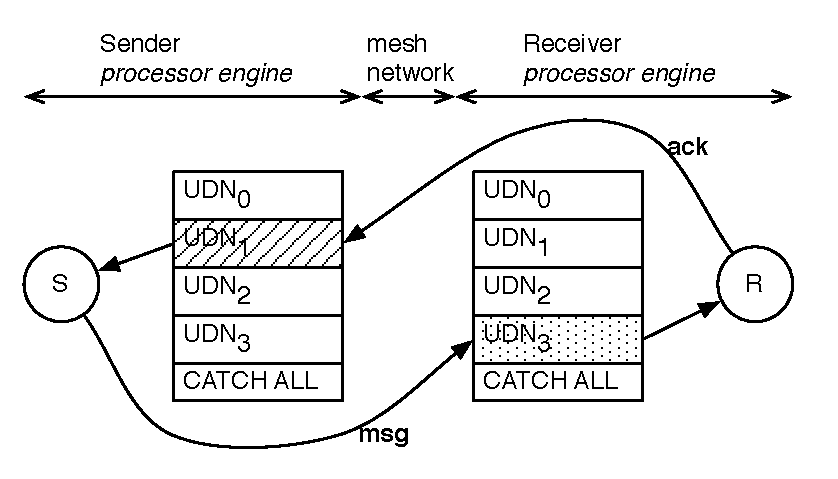
\includegraphics[scale=.5]{udn_sym.pdf}
  \caption[Comunicazione simmetrica su UDN]{Rappresentazione di un possibile scenario di comunicazione simmetrica tra il processo mittente S e quello destinatario R, sfruttando la UDN}
  \label{fig:udn_sym}
\end{figure}
Viene descritta l'implementazione della comunicazione simmetrica che sfrutta in modo ottimale la UDN. 
Tale implementazione pone alcuni limiti sull'utilizzo dei canali ma fornisce le migliori prestazioni possibli riguardo allo scambio dei messaggi sfruttando la UDN. Il protocollo Rdy-Ack per un canale simmetrico viene realizzato impiegando una coda UDN in entrambi i PE che eseguono i processi comunicanti. La coda firmware nel destinatario \`e usata per ricevere i messaggi, il segnale di Rdy \`e implicito con la ricezione di un nuovo messaggio, la coda firmware nel mittente \`e usata per i segnali di Ack, i quali sono esplicitati con l'invio di un messaggio di valore arbitrario di dimensione una parola dal destinatario a tale coda UDN nel mittente. Un possibile scenario \`e mostrato in figura~\ref{fig:udn_sym} dove il canale di comunicazione \`e implementato tramite l'utilizzo della seconda coda UDN nel processo mittente, per la ricezione dei segnali di Ack, e con la quarta coda UDN nel processo destinatario, per la ricezione dei messaggi; ne segue che in entrambi i PE, che eseguono esclusivamente il processo mittente o quello destinatario, rimangono disponibili altre tre code (o canali) UDN utilizzabili per altrettanti canali di comunicazione tra processi. Il protocollo di comunicazione segue quindi lo schema del codice~\ref{lst:abstr_udn_sym}: viene usata una struttura dati condivisa in memoria, il descrittore di canale, acceduta in sola lettura da entrambi i processi comunicanti, contenente l'identificatore delle cpu in cui i processi comunicanti sono eseguiti, e l'identificatore delle code UDN nei due PE, utilizzate dal canale per la comunicazione. La correttezza del protocollo si ottiene con due condizioni: \begin{inparaenum}[\itshape a~\upshape)] \item l'inizializzazione di un canale di comunicazione Rdy-Ack prevede l'invio del segnale di Ack al mittente all'avvio dell'applicazione, in questo caso deve essere inviata una parola arbitraria alla coda UDN usata nel canale dal processo mittente, \item un corretto uso da parte dell'utente dei canali nell'assegnazione delle code UDN a diversi canali di comunicazione: se un canale di comunicazione fa uso di una certa coda UDN, tale coda UDN non deve essere utilizzata da altri canali o da altri meccanismi.\end{inparaenum}
\begin{lstlisting}[
        float=t,
        morekeywords={dq_snd, dq_rcv, cpu_snd, cpu_rcv}, 
        caption={Descrizione astratta del protocollo di comunicazione Rdy-Ack su UDN per un canale di comunicazione simmetrico},
        label={lst:abstr_udn_sym}
]
send(ch_descr, msg) ::
  leggi una parola dalla UDN Demux Queue ch_descr->dq_snd
  invia tramite UDN il valore msg alla UDN Demux Queue 
    ch_descr->dq_rcv del PE ch_descr->cpu_rcv

receive(ch_descr) ::
  leggi una parola dalla UDN Demux Queue ch_descr->dq_rcv e
    assegna il valore alla variablie targa
  invia tramite UDN una parola arbitraria alla UDN Demux
    Queue ch_descr->dq_snd del PE ch_descr->cpu_snd
\end{lstlisting}

L'implementazione descritta limita perci\`o l'uso di questo tipo di canali ad un massimo di quattro canali per processo, l'implementazione bypassa completamente la memoria se non per accedere in sola lettura alle informazioni del canale, la trasmissione dei dati e la sincronizzazione dei processi/PE avviene a livello firmware grazie alla rete di interconnessione e alle primitive di accesso ad essa fornite dal sistema come letture e scritture su registri generali. 

Con il grado di asincronia unitario non esistono problemi di deadlock in quanto, se verificate le condizioni di correttezza, il protocollo garantisce la corretta sincronizzazione e i dati scambiati nella rete sono lunghi una sola parola, quindi non causano l'overrun delle code UDN.

\FloatBarrier
\subsubsection{Comunicazione asimmetrica in ingresso}
\label{sct:asym_udn}
\begin{figure}[!t]
  \centering
  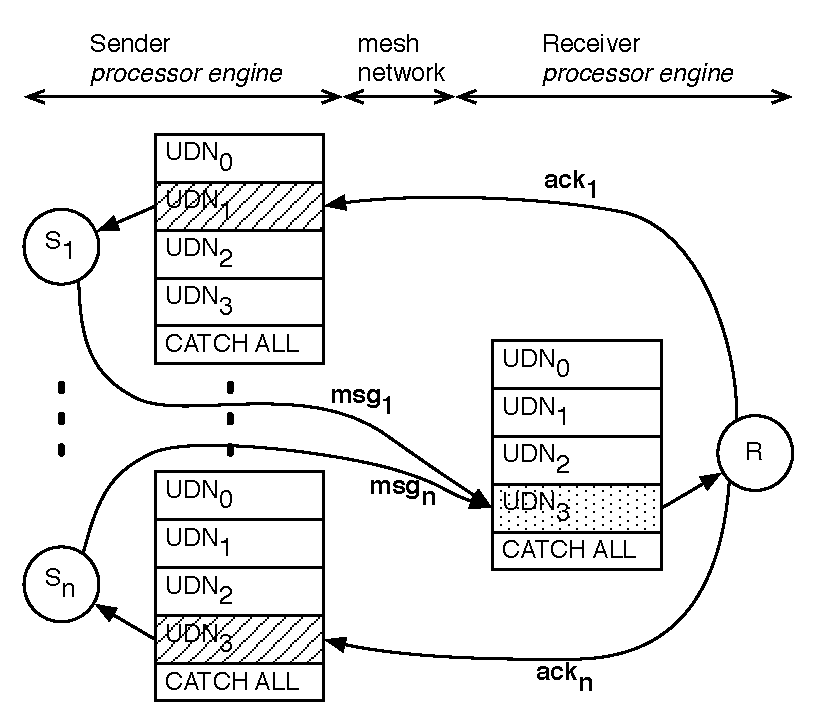
\includegraphics[scale=.5]{udn_asym.pdf}
  \caption[Comunicazione asimmetrica su UDN]{Rappresentazione di un possibile scenario di comunicazione asimmetrica in ingresso tra l'insieme di processi mittenti $\{ S_1, \dots, S_n \}$ e il processo destinatario R, sfruttando la UDN}
  \label{fig:udn_asym}
\end{figure}
L'implementazione della comunicazione asimmetrica in ingresso deriva da quella simmetrica: un generico processo mittente del canale dispone di una coda UDN sulla quale legge gli eventi di Ack, il processo ricevente del canale usa una singola coda UDN sulla quale legge il messaggio di uno qualsiasi tra i processi mittenti. Un messaggio inviato da un mittente \`e costituito da una coppia di valori: una parola di intestazione contenente l'identificatore del mittente all'interno del canale, e una seconda parola contente il valore del messaggio per il quale \`e stato richiesto l'invio. Il fatto che sia trasmesso anche una intestazione al messaggio \`e trasparente all'utente, in quanto l'esecuzione della ricezione nel processo destinatario rende visibile all'utente solo il valore del messaggio. Come mostrato in figura~\ref{fig:udn_asym} diversi mittenti dello stesso canale possono avere come una coda UDN di ricezione qualsiasi, questo crea un problema simile a quello visto nell'implementazione che sfrutta la memoria condivisa nella sezione~\ref{sct:asymin_sm_rdyack}: durante l'esecuzione della primitiva di invio del canale, da parte di un generico mittente, deve essere noto l'identificatore del mittente all'interno del canale stesso, in modo da sapere quale coda UDN usare per l'evento Ack e che valore dare all'intestazione dei messaggi. Anche per questa implementazione del canale asimmetrico si usa un terzo parametro nella primitiva di invio: l'identificatore nel canale del mittente. Il comportamento del protocollo \`e descritto nel codice~\ref{lst:abstr_udn_asym}; come nel canale simmetrico, il supporto fa uso di un descrittore di canale contenente le informazioni sulle cpu e le code UDN usate dai processi comunicanti, nel caso dei processi mittenti tali informazioni sono organizzate in array accedute con l'identificatore del mittente all'interno del canale.
\begin{lstlisting}[
        float=!h,
        morekeywords={dq_snd, dq_rcv, cpu_snd, cpu_rcv}, 
        caption={Descrizione astratta del protocollo di comunicazione Rdy-Ack su UDN per un canale di comunicazione asimmetrico in ingresso},
        label={lst:abstr_udn_asym}
]
send(ch_descr, msg, rank) ::
  leggi una parola dalla UDN Demux Queue 
    ch_descr->dq_snd[rank]
  invia tramite UDN la sequenza di valori <rank, msg> alla
    UDN Demux Queue ch_descr->dq_rcv del PE
    ch_descr->cpu_rcv

receive(ch_descr) ::
  leggi una parola dalla UDN Demux Queue ch_descr->dq_rcv e
    assega il valore alla variablie sender
  leggi una parola dalla UDN Demux Queue ch_descr->dq_rcv e
    assegna il valore alla variablie targa
  invia tramite UDN una parola arbitraria alla UDN Demux
    Queue ch_descr->dq_snd[sender] del PE 
    ch_descr->cpu_snd[sender]
\end{lstlisting}

L'analisi della correttezza della comunicazione \`e simile a quella descritta nell'implementazione simmetrica: \begin{inparaenum}[\itshape a~\upshape)] \item durante l'implementazione del canale devono essere inviati i messaggi di Ack a tutti i mittenti nelle relative code UDN, \item l'utente si fa carico di non usare in un certo processo, eseguito in modo esclusivo in un PE, la stessa coda UDN per pi\`u canali o compiti diversi\end{inparaenum}. Si osserva inoltre che l'unit\`a di routing di UDN \`e il pacchetto \cite{ug101}, quindi l'invio della coppia di parole $<sender_{rank},\;msg>$ da parte di un mittente non viene mai ricevuta intervallata da altre parole nella coda UDN del destinatario se l'invio \`e stato fatto impostando la coppia di parole come payload di un unico pacchetto. Al contrario l'invio di due pacchetti UDN per l'invio della coppia risulta non corretto per l'implementazione descritta.

Si analizza infine la possibilit\`a di situazioni di deadlock causate dall'uso della UDN, che come descritto nella sezione~\ref{sct:intro_arch_udn} \`e soggetta a tale problema. Anche in questo caso l'uso di un paradigma di comunicazione client-server, con un protocollo caratterizzato da grado di asincronia unitario nega il verificarsi di qualsiasi situazione di deadlock (con le ipotesi di correttezza precedenti). Il supporto della comunicazione \`e infatti caratterizzato da un comportamento client-server con interazione domanda-e-risposta, in cui il servente \`e il destinatario e i mittenti sono i clienti. Le richieste dei clienti sono i messaggi inviati dai clienti e le risposte sono i messaggi di ack inviati dal destinatario. In una computazione di questo tipo il deadlock avviene soltanto se i messaggi di risposta del servente riempono la coda di un cliente, ci\`o accade solo quando un cliente invia pi\`u richieste della capacit\`a della coda UDN di memorizzare le risposte \cite{ug205}.

\FloatBarrier
\subsubsection{Comunicazioni con grado di asincronia maggiore di 1}
\label{sct:ad_gt_1_udn}
Le due implementazioni dei canali simmetrici e asimmetrici che sfruttano UDN si prestano ad essere estese ad un grado di asincronia maggiore di uno, \`e infatti sufficiente inviare un numero $m > 1$ di messaggi di Ack al/i mettente/i in fase di inizializzazione del canale. In questo modo eseguendo lo stesso protocollo precedentemente definito si ha un comportamento asincrono di grado $m$. 

Occorre porre attenzione al fatto che un grado di asincronia elevato pu\`o causare il deadlock dell'applicazione. In particolare un mittente non deve inviare pi\`u messaggi della dimensione della coda di demultiplexing UDN. Dato che in entrambe le forme di canale le risposte del destinatario hanno dimensione una parola allora il massimo grado di asincronia \`e la dimensione delle code UDN, per entrambi i canali.

\FloatBarrier
\subsubsection{Implementazione generica}
\label{sct:generic_udn}
Non \`e fornita una implementazione dei canali che sfrutti la UDN e che non limiti per ogni processo il numero di canali utilizzabili. Si descrive qui una possibile implementazione. La limitazione fisica di un numero finito di canali UDN \`e superata utilizzando, con il paradigma precedente, per pi\`u canali ``software'', almeno una coda UDN nel mittente e nel destinatario. I diversi canali ``software'' sono riconosciuti mediante una intestazione ai dati scambiati contenente l'identificatore del canale. \`E necessario ricorrere alla memoria condivisa nel caso in cui il processo destinatario invochi la ricezione su un certo canale e i dati ricevuti dalla coda UDN siano appartenenti ad un altro canale ``software'', perci\`o si memorizzano tali dati per un utilizzo successivo e si continua a testare la coda UDN in attesa dei dati del canale usato. 

Si suppone che una implementazione di questo tipo sia sempre usata insieme all'implementazione ``specializzata su UDN'', pu\`o essere quindi conveniente lasciare le quattro code UDN di demultiplexing a quest'ultima implementazione, e usare la coda \emph{catch all} per l'implementazione ``generica su UDN''. Tale coda viene usata quando si inviano pacchetti UDN con tag di demultiplexing diverso dai quattro valori delle code firmware, la ricezione viene effettuata mediante la lettura di registri SPR. 

L'uso di una implementazione ``UDN generica'' pu\`o essere una utile alternativa alla implementazione che sfrutta esclusivamente la memoria condivisa (descritta in \ref{sct:specifica_sm}) per applicazioni che necessitano di pi\`u di quattro canali per processo e basse latenze di comunicazione. Si osserva tuttavia che pi\`u sono usati molti canali di comunicazione in un singolo processo, pi\`u aumenta la probabilit\`a di ricevere il messaggio di un canale diverso e quindi la necessit\`a di eseguire una copia in memoria (overhead).
